\chapter{Propuesta}\label{chapter:proposal}

\newcommand{\dfscaption}{\hyperref[algo:dfs]{DFS-Votos}}
\newcommand{\cyclevotescaption}{\hyperref[algo:votes-cycles]{Reasignar-Votos-en-Todos-los-Ciclos}}
\newcommand{\dfsvisitcaption}{\hyperref[algo:dfs-visit]{DFS-Votos-Visita}}
\newcommand{\initdfsvertices}{\hyperref[algo:init-dfs-vertices]{Inicializar-Propiedades-de-V\'ertices}}
\newcommand{\maxincyclecaption}{\hyperref[algo:max-in-cycle]{M\'ax-Votos-en-Ciclo}}
\newcommand{\setvotestoallincyclecaption}{\hyperref[algo:set-votes-all-in-cycle]{Reasignar-Votos-en-Ciclo}}

\todo[inline]{@TODO introducir los aspectos fundamentales de la propuesta: conteo d votos y desempate}

\section{Conteo de Votos}
\todo[inline]{@TODO resumir d lo q vas a hablar: contar con DFS en el grafo inverso al d los votos}
Sean $V$ el conjunto de los participantes  de la elecci\'on (votantes) y $f \in V \times V$ la relaci\'on de voto, esto es, $ \langle x, y \rangle \in f $ si y s\'olo si $x$ vot\'o por $ y $.  Se asume que culmin\'o el registro de todos los votos y que s\'olo existen votos v\'alidos. Cada votante puede elegir a lo sumo a otra persona, por ende, $f$ es funci\'on.

Sea $G' = \langle V, f \rangle$ el digrafo de votaci\'on, con v\'ertices en $V$ y arcos en $f$. Representaciones de este grafo pueden ser encontradas en las figuras~\ref{fig:r-voting}~y~\ref{fig:voting-cycle}. \todo[inline]{@FIXME en esas figuras las flechas tienen peso y referenciarlas en este momento puede hacer pensar al lector q el grafo es ponderado}

Ahora bien, sea $G = \langle V, f^{-1} \rangle$ el digrafo que resulta de invertir los arcos de $G'$. Se denota por $G_\pi$ a cualquiera de los subgrafos  de predecesores de un recorrido DFS sobre $G$ \citep{intro-to-algo-3}. El conteo de los votos obtenidos por $x$ se reduce a contar la cantidad de nodos en el sub\'arbol de $x$ en $G_\pi$. \todo{@BUG mentira. El del introduction so'lo setea $\pi$ cuando $v$ es gris}

\todo[inline]{@NOTE cada vez q digas algo q lleve demostracio'n, pon una referencia al lema/teorema q lo respalda en la subseccio'n d correctitud}

El conteo de los votos puede entonces ser implementado mediante DFS. Los algoritmos~\ref{algo:dfs}~y~\ref{algo:dfs-visit}  constituyen adaptaciones   de las funciones DFS y DFS-Visit de \cite{intro-to-algo-3}, respectivamente. Se asume que $G$ se encuentra representado mediante listas de adyacencia. En $B$ se almacenan los arcos de retroceso de $G$.    Una vez el algoritmo~\ref{algo:dfs} termine, en $u.votos$ se tiene la cantidad de votos obtenidos por el votante representado mediante el v\'ertice $u$. A todos los votantes en alg\'un ciclo se les reasignan votos bajo un criterio justo.

\begin{algorithm}[!h]
    \caption{\dfscaption}
    \label{algo:dfs}
    \DontPrintSemicolon
    \SetAlgoLined
    \Entrada{Grafo $G = \langle V, f^{-1} \rangle$.}
    \BlankLine

    \initdfsvertices($G.V$)\;
    $B = \{\}$\;
    \ForEach{v\'ertice $u \in G.V$}{
        \If{$u.color == $ {\rm BLANCO}}{
            \dfsvisitcaption($G, u, B$)\;
        }
    }
    \cyclevotescaption($G, B$)\; \label{algo:dfs:line:votes-in-cycles}
\end{algorithm}

En \dfscaption \;primero se inicializan las propiedades de los v\'ertices. En el algoritmo~\ref{algo:init-dfs-vertices} se pueden observar esas propiedades. La propiedad $votos$ almacena la cantidad de votos recibidos por el v\'ertice. Como se puede apreciar,  \dfscaption \;difiere en muy pocos aspectos a la funci\'on DFS de \cite{intro-to-algo-3}. Uno de los m\'as significativos es el llamado a la funci\'on \cyclevotescaption \;en la l\'inea~\ref{algo:dfs:line:votes-in-cycles}. Esta funci\'on se encarga de reasignar una cantidad justa de votos a cada uno de los v\'ertices que se encuentran en un ciclo.  

\begin{algorithm}[!h]
    \caption{\initdfsvertices}
    \label{algo:init-dfs-vertices}
    \DontPrintSemicolon
    \SetAlgoLined
    \Entrada{Conjunto de v\'ertices $V$.}
    \BlankLine

    \ForEach{v\'ertice $u \in V$}{
        $u.color =$ BLANCO\;
        $u.votos = 0$\;
    }
\end{algorithm}

El algoritmo~\ref{algo:dfs-visit} calcula los votos obtenidos por $u$ y a\~nade a $B$ los arcos de retroceso encontrados durante el proceso.

\begin{algorithm}[!h]
    \caption{\dfsvisitcaption}
    \label{algo:dfs-visit}
    \DontPrintSemicolon
    \Entrada{Grafo $G$; v\'ertice $u$; conjunto $B$ de arcos de retroceso.}     
    \BlankLine

    $u.color =$ GRIS\;

    \ForEach{$v \in G.Adj[u]$}{ \label{algo:dfs-visit:line:arc-foreach}
        \If{$v.color ==$ {\rm BLANCO}}{
            \dfsvisitcaption($G, v, B$)\;
        }\lElse{\If{$v.color ==$ {\rm GRIS}}{
            $B = B \cup \{\langle u, v \rangle\}$\; \label{algo:dfs-visit:line:add-B}
        }}
        \If{$v.color ==$ {\rm NEGRO}}{ \label{algo:dfs-visit:line:if-black}
            $u.votos = u.votos + v.votos + 1$\; \label{algo:dfs-visit:line:votes}
        }
        \label{algo:dfs-visit:line:if-black:end}
    }
    \label{algo:dfs-visit:line:arc-foreach:end}
    $u.color =$ NEGRO\;
\end{algorithm}

El ciclo de las l\'ineas~\ref{algo:dfs-visit:line:arc-foreach}-\ref{algo:dfs-visit:line:arc-foreach:end} itera por todos los arcos salientes de $u$. N\'otese que $v \in G.Adj[u]$ si y s\'olo si $v$ vot\'o por $u$, por definici\'on de $G$.  Se a\~nade un nuevo arco de retroceso a $B$ en la l\'inea~\ref{algo:dfs-visit:line:add-B}. Un arco $\langle u, v \rangle$ es de retroceso si y s\'olo si $v$ es gris cuando se explora ese arco por primera vez \citep{intro-to-algo-3}. El n\'umero de votos obtenidos por $u$ es actualizado solamente en la l\'inea~\ref{algo:dfs-visit:line:votes}, cuando $v$ es negro. Esto se debe a que los votos obtenidos por $v$ se encuentran bien calculados cuando este es negro. Todos los votos obtenidos por $v$, m\'as el voto que este le confiere a $u$, son contados como votos de  $u$. N\'otese que el bloque de las l\'ineas~\ref{algo:dfs-visit:line:if-black}-\ref{algo:dfs-visit:line:if-black:end} es un ``\textbf{si}'', y no un ``\textbf{en otro caso si}''. Esto es intencional y permite que se actualicen los votos de $u$ correctamente, incluso cuando $\langle u, v \rangle$ es un arco de \'arbol de $G_\pi$. 

\todo[inline]{@TODO probar q cuan2 v es negro entonces los votos d v esta'n bien contados}

El algoritmo~\ref{algo:votes-cycles} considera todos los ciclos de $G$. En cada iteraci\'on, se calcula el mayor n\'umero de votos obtenidos por un v\'ertice del ciclo y le asigna esa cantidad a los restantes v\'ertices del propio ciclo. Los votantes de un mismo ciclo conf\'ian indirectamente entre ellos dos a dos, por ende, se considera justo que cada uno de ellos obtenga la misma cantidad de votos, y que esta sea la mayor obtenida por un miembro del ciclo.


\begin{algorithm}[!h]
    \caption{\cyclevotescaption}
    \label{algo:votes-cycles}
    \DontPrintSemicolon
    \SetAlgoLined
    \Entrada{Grafo $G = \langle V, f^{-1} \rangle$; conjunto $B$ de arcos de retroceso.}     
    \BlankLine

    \ForEach{$\langle u, v \rangle \in B$}{
        $m = $ \maxincyclecaption($\langle u, v \rangle, f$)\;
        \setvotestoallincyclecaption($m, \langle u, v \rangle, f$)\;
    }
\end{algorithm}

\todo[inline]{@TODO hay q probar q c esta'n considerando todos los ciclos}

Dado un arco de retroceso $\langle u, v \rangle$ y la funci\'on de votaci\'on $f$, \maxincyclecaption \;itera por todos los v\'ertices del ciclo al que ese arco pertenece, mediante m\'ultiples aplicaciones de $f$. El algoritmo devuelve la mayor cantidad de votos obtenidos por alg\'un v\'ertice del ciclo. 

\begin{algorithm}[!h]
    \caption{\maxincyclecaption}
    \label{algo:max-in-cycle}
    \DontPrintSemicolon
    \SetAlgoLined
    \Entrada{Arco de retroceso $\langle u, v \rangle$; funci\'on de votaci\'on $f$.}     
    \Salida{Mayor n\'umero de votos obtenidos por un v\'ertice del ciclo.}
    \BlankLine

    $m = v.votos$\;
    $x = u$\;
    \While{$x \neq v$}{
        $m = \max(m, x.votos)$\;
        $x = f(x)$\;
    }
    \Return{$m$}\;
\end{algorithm}

El algoritmo~\ref{algo:set-votes-all-in-cycle} itera de igual manera por todos los v\'ertices del ciclo al que pertenece el arco de retroceso dado. La cantidad de votos dada ($m$) es asignada a cada v\'ertice de ciclo.

\todo[inline]{@TODO probar q el ciclo de los algoritmos~\ref{algo:set-votes-all-in-cycle}~y~\ref{algo:max-in-cycle} termina}

\begin{algorithm}[!h]
    \caption{\setvotestoallincyclecaption}
    \label{algo:set-votes-all-in-cycle}
    \DontPrintSemicolon
    \SetAlgoLined
    \Entrada{$m$ votos a asignar; arco de retroceso $\langle u, v \rangle$; funci\'on de votaci\'on $f$.}     
    \BlankLine

    $x = u$\;
    \While{$x \neq v$}{
        $x.votos = m$\;
        $x = f(x)$\;
    }
    $v.votos = m$\;
\end{algorithm}

\subsection{Correctitud}
\todo[inline]{@NOTE  antes d tirarte a demostrar algo mira a ver si es necesario o si c puede citar al introduction o a alguna conf d eda, discreta, daa, etc}

El algoritmo~\ref{algo:votes-cycles} itera por todos los arcos de retroceso de $G$, los cuales se encuentran en $B$. Cada uno de ellos pertenece a un ciclo y todo ciclo tiene un arco en $B$. \todo{@TODO demostrar} Basta con un arco de retroceso $\langle u, v \rangle$ y la funci\'on $f$ para hallar todos los arcos del ciclo donde $\langle u, v \rangle$ se encuentra. Las funciones \maxincyclecaption \;y \setvotestoallincyclecaption  \todo{@TODO completar esto}

\subsection{Complejidad Temporal}
\todo[inline]{@TODO complejidad temporal del conteo d votos}


\section{Desempate}
Sean $m = \max\{ u.votos \;|\; u \in V \}$ y $W = \{ u \in V \;|\; u.votos = m \}$.  Si $|W| = 1$, entonces se declara como ganador al \'unico elemento de $W$. Para determinar qui\'en gana cuando $|W| > 1$, se emplea una adaptaci\'on del m\'etodo de desempate instant\'aneo. 

Para utilizar ese m\'etodo es necesario definir (secci\'on~\ref{sec:irv}):
\begin{enumerate}
    \item un \textit{ranking} de votaci\'on para cada votante, y
    \item una manera de seleccionar qu\'e candidato eliminar en cada ronda, en caso de que m\'as de uno  obtenga la menor cantidad de votos.
\end{enumerate}  

\subsection{\textit{Rankings}}
Sea $x \in V$ un v\'ertice cualquiera de $G'$. Sea $P(x)$ un camino simple maximal de $G'$ que comienza en $x$. Luego,
$$
P(x) = \langle x, f(x), f(f(x)), \ldots, f^{k}(x) \rangle.
$$
Como $f$ es funci\'on, entonces $P(x)$ es \'unico. 

El \textit{ranking} de $x$ se define como  la subsecuencia maximal de $P(x)$ de v\'ertices distintos de $x$ que est\'an en $W$. El orden en el que aparecen los votantes en el \textit{ranking} es el mismo que el orden en el que aparecen en la subsecuencia.

En la figura~\ref{fig:graph-13-voters-2-cycles} se representa un grafo de votaci\'on con 13 votantes y 2 ciclos.

\begin{figure}[h!]
    \centering
    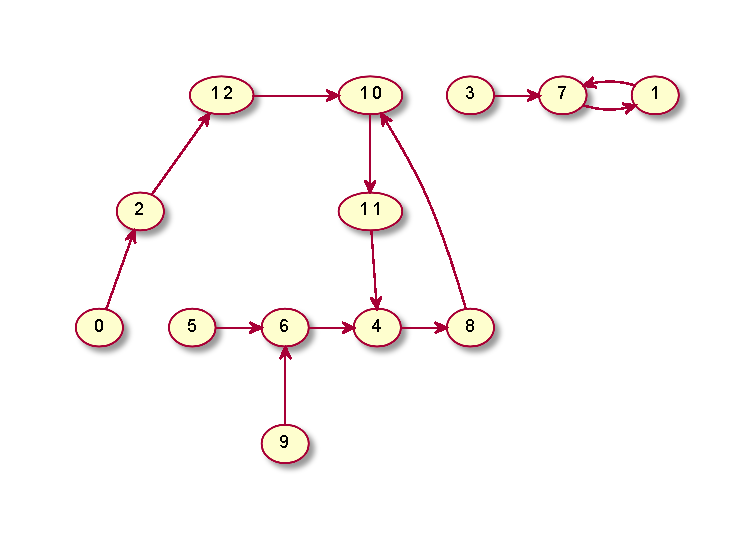
\includegraphics[scale=.9]{Graphics/graph-13-voters-2-cycles-largest-has-4.pdf}
    \caption{Grafo de votaci\'on con 13 votantes y 2 ciclos.}
    \label{fig:graph-13-voters-2-cycles}
\end{figure}

En ese caso, se tiene que $m = 9$ y $W = \{ 4, 8, 10, 11 \}$. En la tabla~\ref{tab:rankings-13-voters} se muestran los \textit{rankings} de cada votante.

\begin{table}[h!]
    \centering
    \begin{tabular}{|c|c|c|c|c|c|c|c|c|c|c|c|c|c|}
        \hline
        posici\'on/votante & 0  & 1  & 2  & 3  & 4  & 5  & 6  & 7  & 8  & 9  & 10 & 11 & 12 \\ \hline
        1                  & 10 &    & 10 &    & 8  & 4  & 4  &    & 10 & 4  & 11 & 4  & 10 \\ \hline
        2                  & 11 &    & 11 &    & 10 & 8  & 8  &    & 11 & 8  & 4  & 8  & 11 \\ \hline
        3                  & 4  &    & 4  &    & 11 & 10 & 10 &    & 4  & 10 & 8  & 10 & 4  \\ \hline
        4                  & 8  &    & 8  &    &    & 11 & 11 &    &    & 11 &    &    & 8  \\ \hline
    \end{tabular}
    \caption{Ejemplo de \textit{rankings} para 13 votantes (ver figura~\ref{fig:graph-13-voters-2-cycles}).}
    \label{tab:rankings-13-voters}
\end{table}

N\'otese que los \textit{rankings}  de los votantes 1, 3 y 7 est\'an vac\'ios, ya que no existe un camino en el grafo desde alguno de ellos hacia un v\'ertice de $W$.

\subsection{Eliminando por Tiempo}
Cuando en una ronda de IRV dos o m\'as candidatos poseen la menor cantidad de votos, es preciso decidir a cu\'al de ellos eliminar. Se propone eliminar al que obtuvo esa cantidad de votos m\'as tarde en el tiempo. La propuesta se basa en la hip\'otesis de que si un candidato obtuvo sus votos en menos tiempo que otro, entonces los votantes del primero poseen m\'as seguridad y confianza en su elecci\'on que los votantes del segundo. Esta hip\'otesis se hace m\'as fuerte cuando es menos el conocimiento que poseen los votantes sobre los candidatos antes de que comience la elecci\'on. 
\todo[inline]{@TODO propo'n una manera d minimizar ese conocimiento o mira a ver si precisamente esa es una caracter\'istica del problema}

A continuaci\'on se formaliza la propuesta.


Cada voto se registra en el sistema en un tiempo determinado. Sea $t(x)$ el tiempo en el que el voto de $x$ es registrado. $t$ es funci\'on, ya que de cada persona se puede registrar a lo sumo un voto v\'alido. Esta funci\'on est\'a indefinida para las personas que no votaron.

Si antes de la primera ronda de IRV $y$ aparece en el \textit{ranking} de $x$, entonces $y = f^r(x)$, o sea, existe una secuencia de v\'ertices $x = p_1, p_2, ..., p_{r+1} = y$, tal que $p_i$ vot\'o por $p_{i+1}$, para todo $i, 1 \leq i \leq r$. \todo{@TODO referencia a la definicio'n d ranking} Se puede decir que $x$ vot\'o por $y$ directa (si $r=1$) o indirectamente (si $r>1$) y que $y$ obtuvo ese voto en el tiempo $\max (t(p_1), t(p_2), ..., t(p_r))$, el cual se puede denotar por $t_{rank}(x, y)$. 

Si en una ronda cualquiera de IRV, $y$ aparece en la primera posici\'on del \textit{ranking} de $x$, entonces $x$ vot\'o por $y$ directa o indirectamente. En cualquier caso, $t_{rank}(x, y)$ es una definici\'on para el tiempo en que $y$ obtiene ese voto. Sup\'ongase que $y$ se encuentra en la primera posici\'on de los \textit{rankings} de $x_1, x_2, ..., x_s$ en una ronda determinada de IRV. Luego, $y$ tiene $s$ votos en IRV y se dice que los obtuvo en tiempo 

\begin{equation}\label{eq:max-rank-time}
   t_{ronda}(y) = \underset{1 \leq i \leq s}{\max} \{ t_{rank}(x_i, y) \}. 
\end{equation}

Finalmente, de todas las personas con la menor cantidad de votos en una ronda de IRV, se propone eliminar a la que obtuvo sus votos m\'as tarde en el tiempo, esto es, la que tiene mayor valor  de $t_{ronda}$.

\subsubsection{Correctitud}
\todo[inline]{@TODO demostrar q desempata y q IRV termina}

\todo[inline]{@TODO di q se habla indistintamente de persona y ve'rtice desde q modelas este problema como uno de grafo}

\todo[inline]{@TODO di q so'lo hay q tener en cuenta la gente q aparece en algu'n ranking, o sea, a la gente de $W$}
% Formalmente, el \textit{ranking} de $x$ es
% $$
% R(x) = \langle y_{i_1}, y_{i_2}, \ldots, y_{i_t} \rangle, \quad 1 \leq i_1 \leq i_2 \leq \ldots \leq i_t \leq k, \quad y_{i_j} \in W \setminus D, \; 1 \leq \forall j \leq t.
% $$
% Formalmente, el \textit{ranking} de $x$ es
% $$
% R(x) = \langle y_{i_1}, y_{i_2}, \ldots, y_{i_t} \rangle, \quad 1 \leq i_1 \leq i_2 \leq \ldots \leq i_t \leq k, \quad y_{i_j} \in W \setminus D, \; 1 \leq \forall j \leq t.
% $$

% @FIXME change blankspace between (figura|tabla|algoritmo) and (\ref|\cite) command for a ~
% @TODO remove \SetAlgoLined from all algorithms
\todo[inline]{@TODO deja claro a la hora d definir el problema d q cada participante es a la vez votante y candidato para poder hablar indistintamente en es senti2}